\chapter{Signal modeling and systematic uncertainties}
\label{ch:signals}


This search targets three different types of \gammajet resonance signals: \acp{EQ}, \acp{QBH} and generic, Gaussian-shaped resonances. To perform hypothesis tests for these signals, their expected \myj spectra must be known.
These predicted signal shapes are modeled by a continuous \ac{PDF2} that are later included in the \ac{SB} fits.
Also, the theoretical and experimental systematic uncertainties are studied in this chapter, as these enter the final fits performed to data.







%%%%%%%%%%%%%%%%%%%%%%%%%%%%%%%%%%%%%%%%%%%%%%%%%%%%%%%%%%%%%%%%%%%%%%%%%%%%%%%%%%%%%%%%%%%%%%%%%%%%
%%%%%%%%%%%%%%%%%%%%%%%%%%%%%%%%%%%%%%%%%%%%%%%%%%%%%%%%%%%%%%%%%%%%%%%%%%%%%%%%%%%%%%%%%%%%%%%%%%%%
%%%%%%%%%%%%%%%%%%%%%%%%%%%%%%%%%%%%%%%%%%%%%%%%%%%%%%%%%%%%%%%%%%%%%%%%%%%%%%%%%%%%%%%%%%%%%%%%%%%%
%%%%%%%%%%%%%%%%%%%%%%%%%%%%%%%%%%%%%%%%%%%%%%%%%%%%%%%%%%%%%%%%%%%%%%%%%%%%%%%%%%%%%%%%%%%%%%%%%%%%
%%%%%%%%%%%%%%%%%%%%%%%%%%%%%%%%%%%%%%%%%%%%%%%%%%%%%%%%%%%%%%%%%%%%%%%%%%%%%%%%%%%%%%%%%%%%%%%%%%%%
%%%%%%%%%%%%%%%%%%%%%%%%%%%%%%%%%%%%%%%%%%%%%%%%%%%%%%%%%%%%%%%%%%%%%%%%%%%%%%%%%%%%%%%%%%%%%%%%%%%%
\section{Signal modeling}
\label{sec:signals:modeling}

The fully-simulated signal model describes both the invariant mass shape, the efficiency and the signal acceptances. However, these signals are generated in a limited set of masses (and couplings in the case of \acp{EQ} signals), but one would like to evaluate the signal predictions at any intermediate parameter, that is, rely on interpolated signals.

To accomplish this interpolation, a two step process is followed. First, it is necessary that each one of the simulated signals follow a continuous distribution rather than a histogram. This process of transforming a histogram to a \ac{PDF2} was employed in the calculation of \acp{FF}, in \Sect{\ref{subsec:ss_corrections:ffs:calculation}}, but with the purpose of smoothing the histograms. In this case, the \ac{KDE} algorithm is used to retrieve a \ac{PDF2} from the signal histogram.
% and the fine factors are optimised for each signal on the grid.

\begin{figure}[ht!]
    \centering
    \begin{subfigure}[h]{0.49\linewidth}
        \centering
        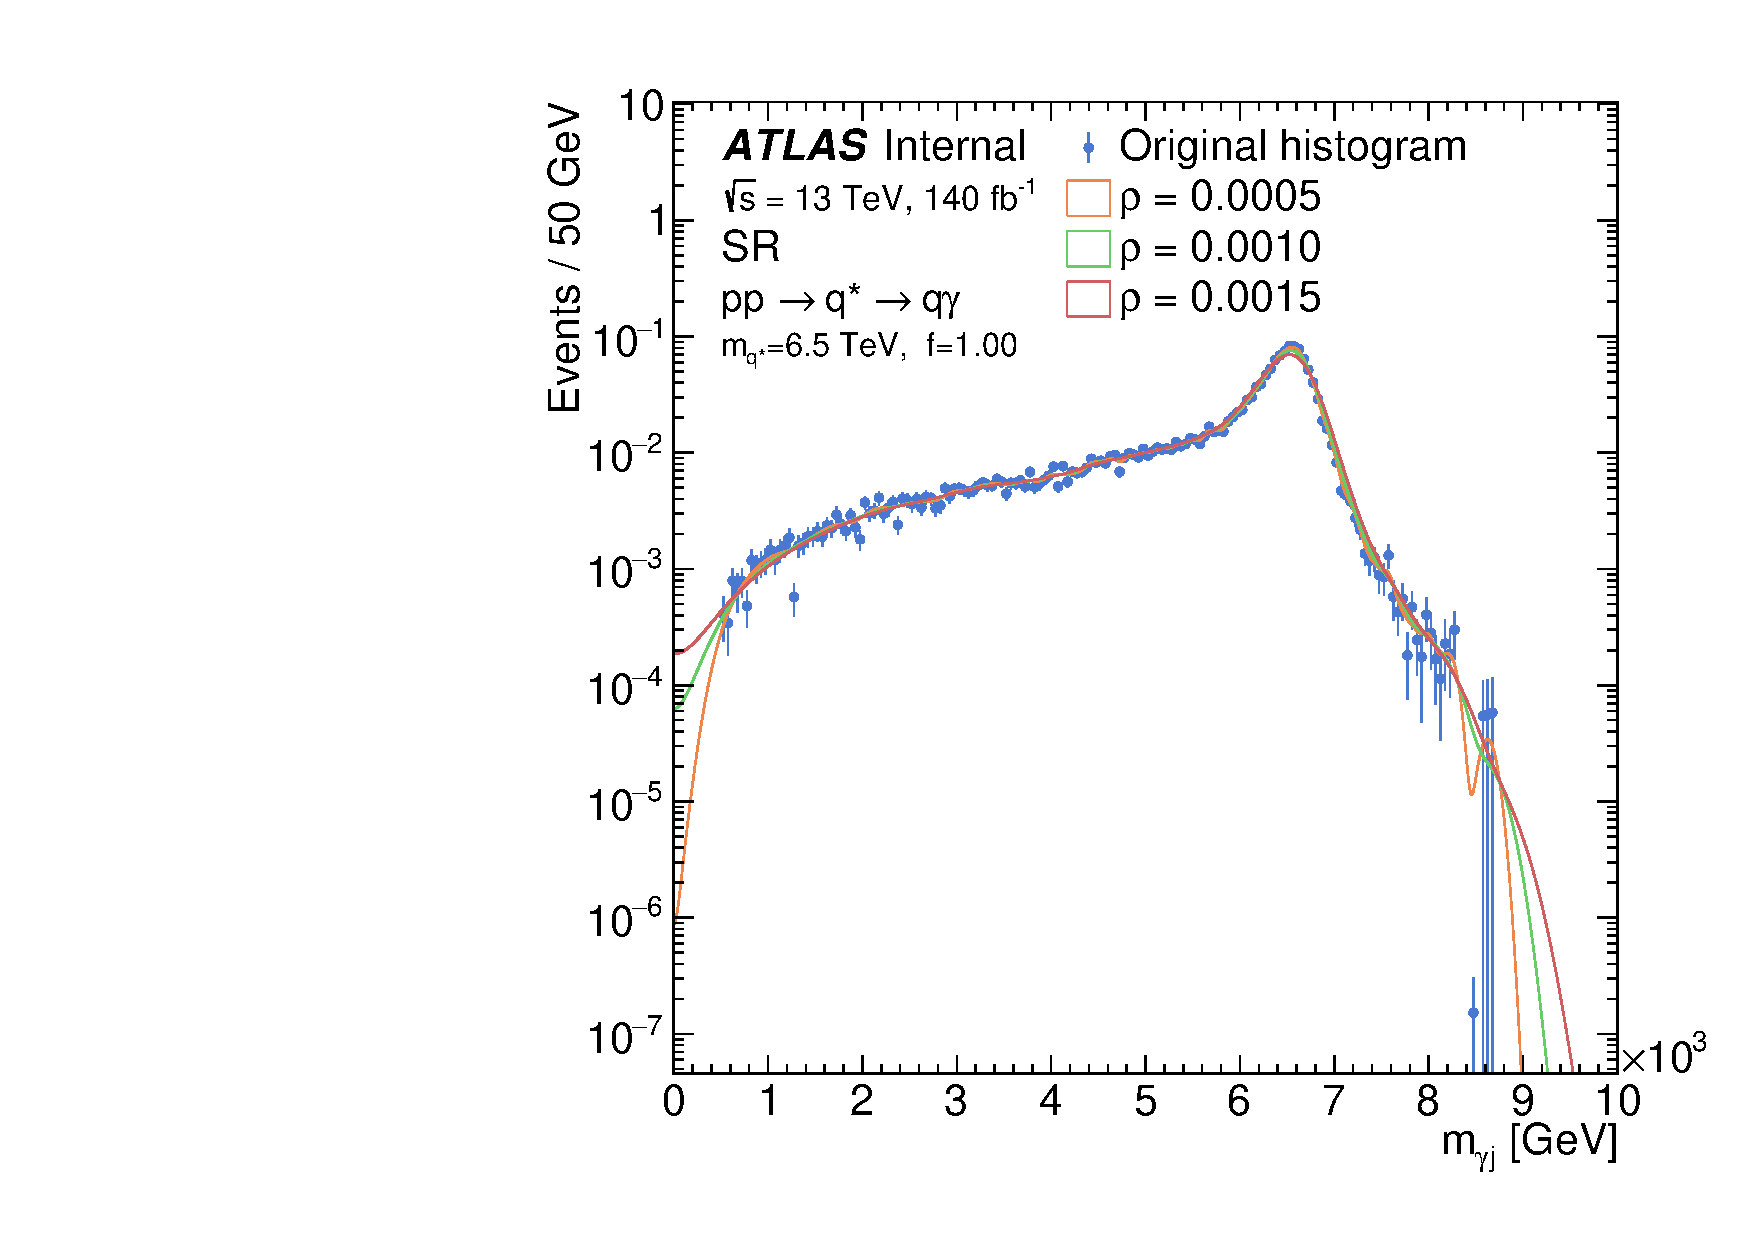
\includegraphics[width=\linewidth]{5_resonances/signal/can__kde_comparison_rhos__qStar_f1p00_M6500__SR}
        \caption{\qstar model with \(\mq = 6500~\gev,\, f=1.0\)}
        \label{fig:signals:modeling:fine_factor_optimization_qstar}
    \end{subfigure}
    \begin{subfigure}[h]{0.49\linewidth}
        \centering
        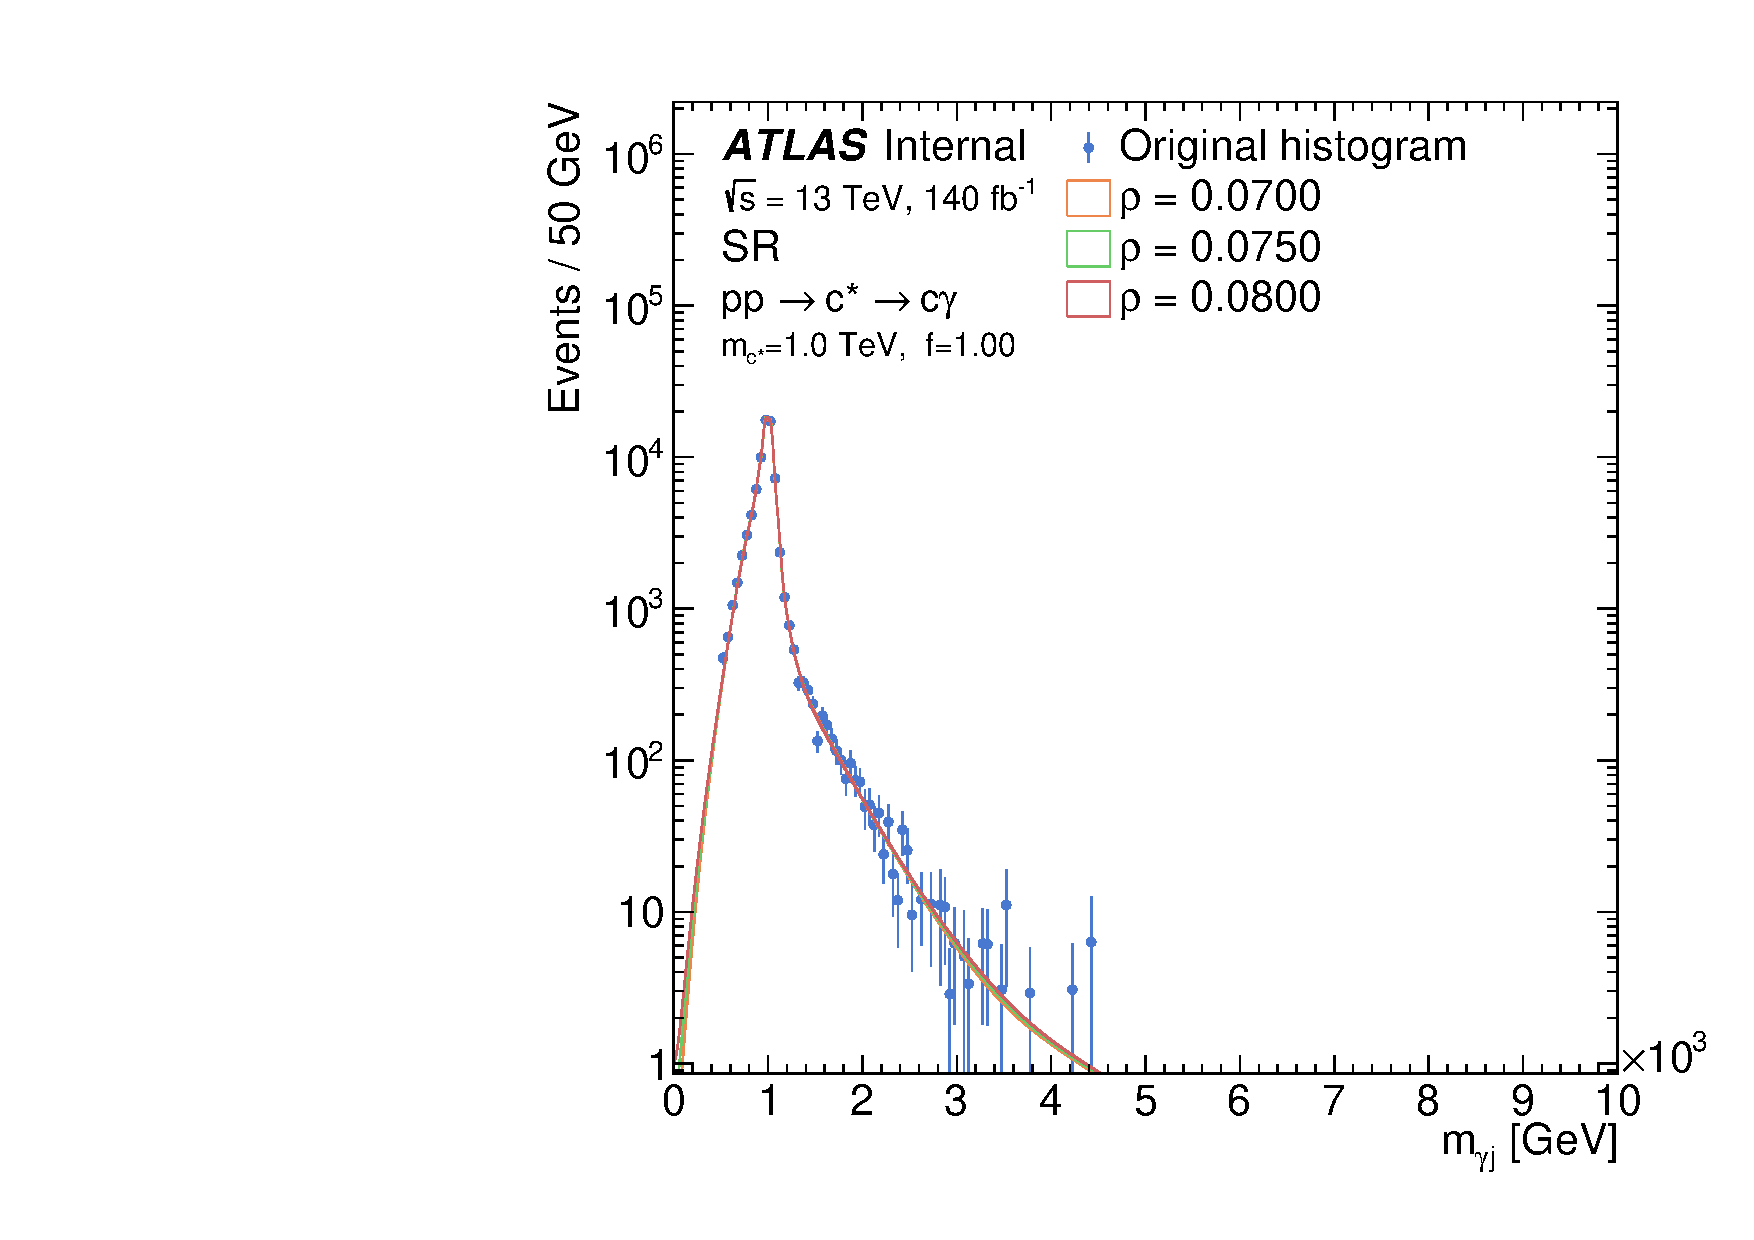
\includegraphics[width=\linewidth]{5_resonances/signal/can__kde_comparison_rhos__cStar_f1p00_M1000__SR}
        \caption{\cstar model with \(\mc = 1000~\gev,\, f=1.0\)}
        \label{fig:signals:modeling:fine_factor_optimization_cstar}
    \end{subfigure}
    \caption{Fine factors optimization for the \qstar and \cstar signal models. Points represents original distribution, while coloured lines represent the estimated \acp{PDF2}.}
    \label{fig:signals:modeling:fine_factor_optimization}
\end{figure}

The fine factors are optimized by eye for parameter of the theory, both for the \ac{EQ} model and \ac{QBH} models. Examples of the optimization can be found on \Fig{\ref{fig:signals:modeling:fine_factor_optimization}} for \qstar and \cstar signals. As the number of entries in the main core of the distributions span multiple orders of magnitude, it is most important to model correctly the peak of the distributions rather than the tails, therefore in some cases the tails are not perfectly modeled for all entries of the original distributions.

Once all the \acp{PDF2} are obtained, signals models for any intermediate mass and/or coupling are obtained with a moment morphing method as described in \Refn{\cite{MomentMorphing}}. The interpolation is done in a pair-wise manner: to obtain any intermediate \ac{PDF2}, the closest two to the desired mass/coupling value are used. For instance, to obtain an interpolated signal with \(\mq = 3200~\gev, \, f=1\), the input signals to the interpolation are the ones with \(\mq = 3000~\gev\) and \(\mq = 4000~\gev\).
This method of obtaining the signal samples is shown in \Fig{\ref{fig:signals:modeling:final_interpolation}}, which contains the interpolated signals with dashed lines and the original ones with solid lines for the \qstar model. For all the interpolated signals, shapes are sensible and lead to a smooth transition between original signal samples.


\begin{figure}[ht!]
    \centering
    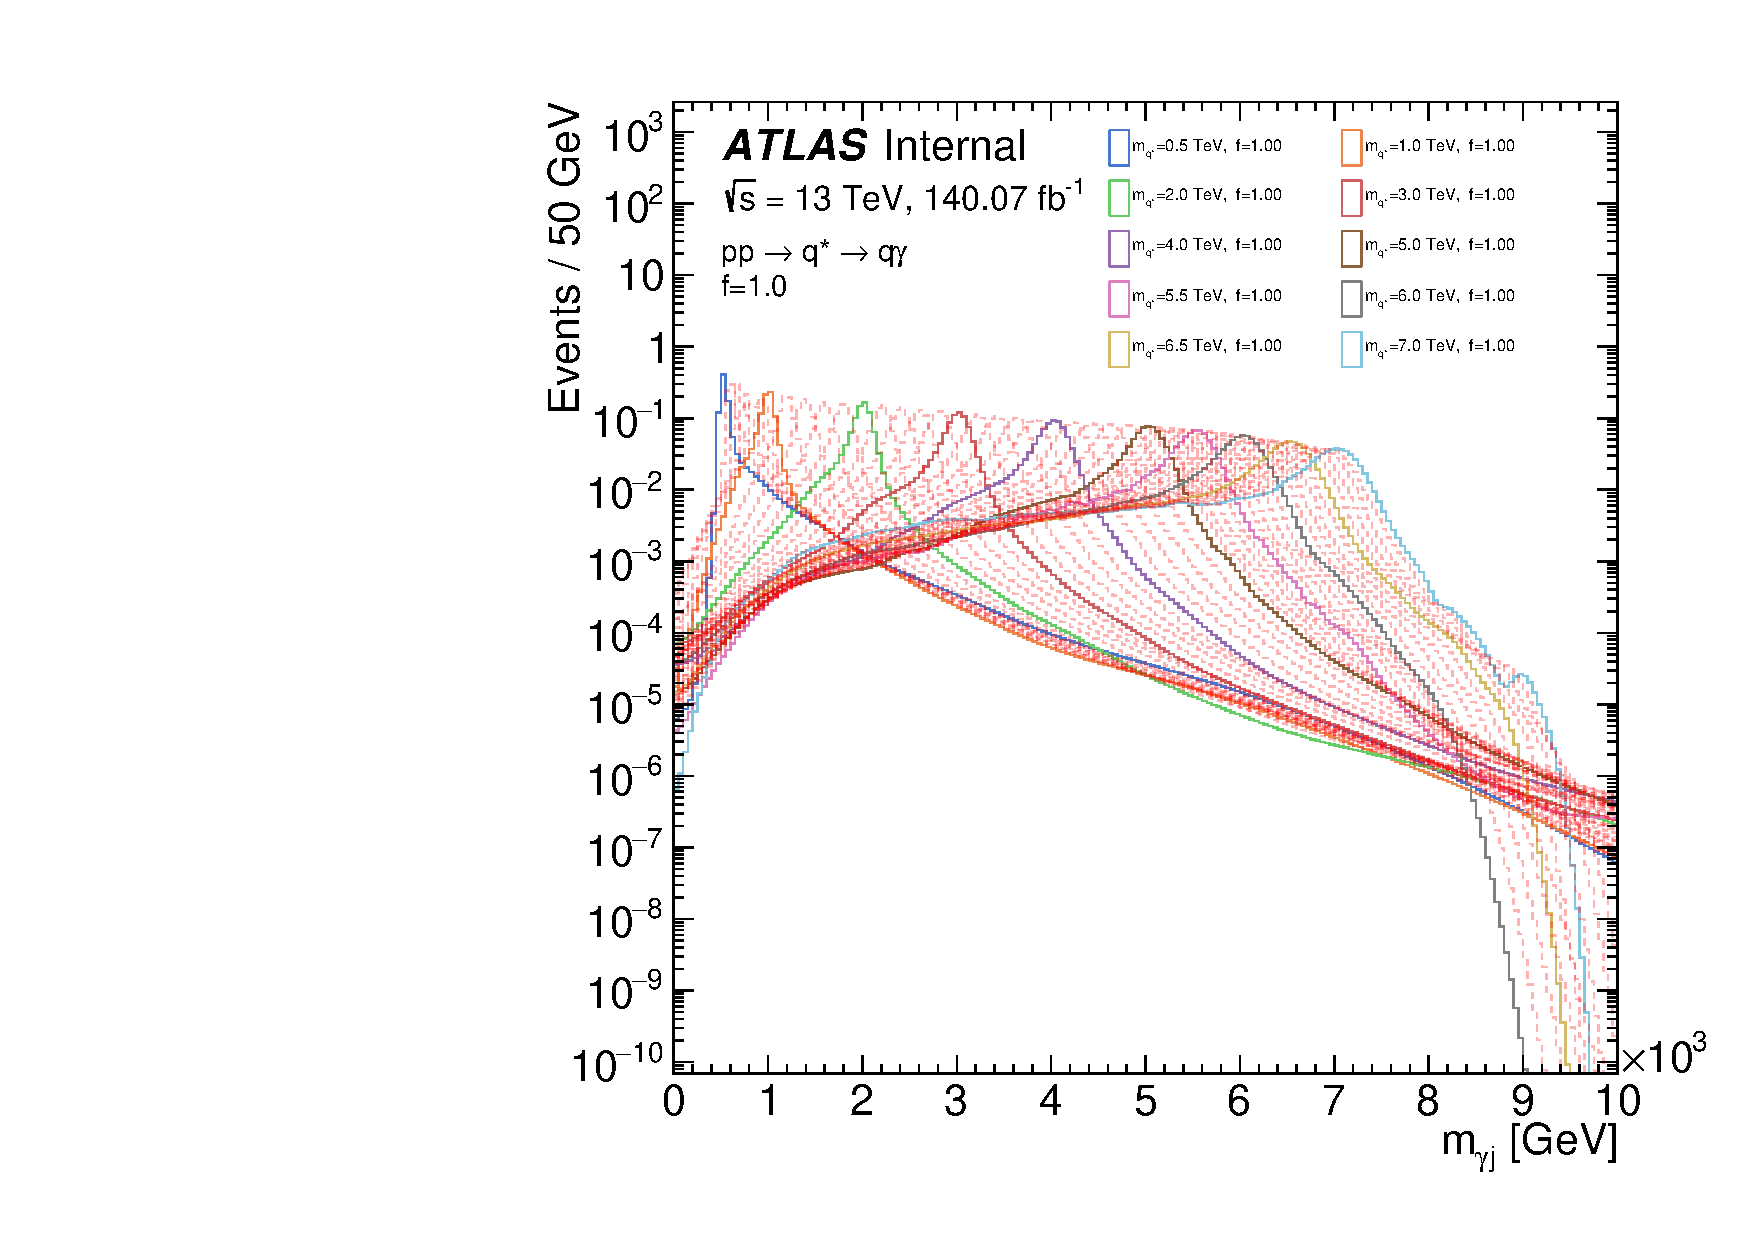
\includegraphics[width=0.6\linewidth]{5_resonances/signal/can__qstar__q_1p00__coupling_interpolation}
    \caption{Illustration of the moment morph method to interpolate between \acp{PDF2}, for the case of \qstar signals with \(f=1\). The original signal distributions are shown with the solid lines with different colors, while all the inteprolated shapes are shown with the dashed red line.}
    \label{fig:signals:modeling:final_interpolation}
\end{figure}
%%%%%%%%%%%%%%%%%%%%%%%%%%%%%%%%%%%%%%%%%%%%%%%%%%%%%%%%%%%%%%%%%%%%%%%%%%%%%%%%%%%%%%%%%%%%%%%%%%%%
%%%%%%%%%%%%%%%%%%%%%%%%%%%%%%%%%%%%%%%%%%%%%%%%%%%%%%%%%%%%%%%%%%%%%%%%%%%%%%%%%%%%%%%%%%%%%%%%%%%%
%%%%%%%%%%%%%%%%%%%%%%%%%%%%%%%%%%%%%%%%%%%%%%%%%%%%%%%%%%%%%%%%%%%%%%%%%%%%%%%%%%%%%%%%%%%%%%%%%%%%
%%%%%%%%%%%%%%%%%%%%%%%%%%%%%%%%%%%%%%%%%%%%%%%%%%%%%%%%%%%%%%%%%%%%%%%%%%%%%%%%%%%%%%%%%%%%%%%%%%%%
%%%%%%%%%%%%%%%%%%%%%%%%%%%%%%%%%%%%%%%%%%%%%%%%%%%%%%%%%%%%%%%%%%%%%%%%%%%%%%%%%%%%%%%%%%%%%%%%%%%%
%%%%%%%%%%%%%%%%%%%%%%%%%%%%%%%%%%%%%%%%%%%%%%%%%%%%%%%%%%%%%%%%%%%%%%%%%%%%%%%%%%%%%%%%%%%%%%%%%%%%










%%%%%%%%%%%%%%%%%%%%%%%%%%%%%%%%%%%%%%%%%%%%%%%%%%%%%%%%%%%%%%%%%%%%%%%%%%%%%%%%%%%%%%%%%%%%%%%%%%%%
%%%%%%%%%%%%%%%%%%%%%%%%%%%%%%%%%%%%%%%%%%%%%%%%%%%%%%%%%%%%%%%%%%%%%%%%%%%%%%%%%%%%%%%%%%%%%%%%%%%%
%%%%%%%%%%%%%%%%%%%%%%%%%%%%%%%%%%%%%%%%%%%%%%%%%%%%%%%%%%%%%%%%%%%%%%%%%%%%%%%%%%%%%%%%%%%%%%%%%%%%
%%%%%%%%%%%%%%%%%%%%%%%%%%%%%%%%%%%%%%%%%%%%%%%%%%%%%%%%%%%%%%%%%%%%%%%%%%%%%%%%%%%%%%%%%%%%%%%%%%%%
%%%%%%%%%%%%%%%%%%%%%%%%%%%%%%%%%%%%%%%%%%%%%%%%%%%%%%%%%%%%%%%%%%%%%%%%%%%%%%%%%%%%%%%%%%%%%%%%%%%%
%%%%%%%%%%%%%%%%%%%%%%%%%%%%%%%%%%%%%%%%%%%%%%%%%%%%%%%%%%%%%%%%%%%%%%%%%%%%%%%%%%%%%%%%%%%%%%%%%%%%
\section{Acceptances and efficiencies}
\label{sec:signals:acc_eff}

The event selection described in the previous chapter is aimed to reduce non-\(s\)-channel \gammajet backgrounds while maintaining a high signal efficiency. In addition to that, the novel GN2 tagger is used to separate the inclusive signal region SR into three orthogonal ones: SRB for \bjets, SRC for \cjets, and SRL for \ljets. This is a crucial aspect in the analysis as it allows, for the first time at the \ac{LHC}, to study \ac{EQ} resonances initiated by a \cstar, orthogonal to other flavors.

\begin{table}[ht!]
    \centering
    \caption{\ac{EQ} signals signifcances over the total background in the SR, SRB, SRC and SRL regions. The considered signals for each flavor have coupling \(f=1.0\).}
    \begin{subtable}[t]{\linewidth}
        \centering
        \caption{\(m = 2000~\gev\) in a window of \(1000<\myj<3000~\gev\)}
        { \tiny
        \begin{tabular}{l >{\raggedleft\arraybackslash}p{0.18\linewidth}>{\raggedleft\arraybackslash}p{0.18\linewidth}>{\raggedleft\arraybackslash}p{0.18\linewidth}>{\raggedleft\arraybackslash}p{0.18\linewidth}}
                \toprule
                \textbf{Signal channel} & SR & SRB & SRC & SRL \\
                \midrule
                Total Bkg. events & 89030.428 & 2570.406 & 14911.838 & 71548.184 \\
                \midrule
                jet \ra $\gamma$ fake   & 3649.795 & 180.319 & 673.710 & 2795.767 \\
                $\gamma$ + jets \Pythia & 85380.633 & 2390.087 & 14238.128 & 68752.418 \\
                \midrule
                \bstar & 242.824, \(Z = 0.810\)    & 147.637, \(Z = 2.880\)  & 40.605, \(Z = 0.330\)    & 54.582, \(Z = 0.200\) \\
                \cstar & 1576.968, \(Z = 5.270\)   & 108.852, \(Z = 2.130\)  & 729.760, \(Z = 5.930\)   & 738.356, \(Z = 2.760\) \\
                \qstar & 31183.749, \(Z = 99.160\) & 625.209, \(Z = 11.880\) & 4335.836, \(Z = 33.970\) & 26222.705, \(Z = 92.810\) \\
                \bottomrule
            \end{tabular}
        }
    \end{subtable}\\
    \smallskip
    \begin{subtable}[t]{\linewidth}
        \centering
        \caption{\(m = 4000~\gev\) in a window of \(3000<\myj<5000~\gev\)}
        { \tiny
            \begin{tabular}{l >{\raggedleft\arraybackslash}p{0.18\linewidth}>{\raggedleft\arraybackslash}p{0.18\linewidth}>{\raggedleft\arraybackslash}p{0.18\linewidth}>{\raggedleft\arraybackslash}p{0.18\linewidth}}
                \toprule
                \textbf{Signal channel} & SR & SRB & SRC & SRL \\
                \midrule
                Total Bkg. events & 200.888 & 5.999 & 27.677 & 167.212 \\
                \midrule
                jet \ra $\gamma$ fake   & 7.014 & 0.334 & 1.419 & 5.260 \\
                $\gamma$ + jets \Pythia & 193.874 & 5.665 & 26.258 & 161.951 \\
                \midrule
                \bstar & 0.708, \(Z = 0.050\) & 0.281, \(Z = 0.110\) & 0.136, \(Z = 0.030\) & 0.291, \(Z = 0.020\) \\
                \cstar & 5.514, \(Z = 0.390\) & 0.337, \(Z = 0.140\) & 1.668, \(Z = 0.310\) & 3.509, \(Z = 0.270\) \\
                \qstar & 295.673, \(Z = 17.530\) & 6.803, \(Z = 2.410\) & 33.739, \(Z = 5.520\) & 255.131, \(Z = 16.500\) \\
                \bottomrule
            \end{tabular}
        }
    \end{subtable}
    \label{tab:signals:acc_eff:qstar_signficances}
\end{table}


In high-energy physics it is fundamental to first study the sensitivity of the signals that are searched for. In \Tab{\ref{tab:signals:acc_eff:qstar_signficances}}, the number of events for each considered background\footnote{The jet-faking-photon background is studied in \Ch{\ref{ch:bkg}}.}, as well as the number of signal events in each of one of the signal regions, for two benchmark signals. The signal regions in the tables, however, have an additional cut on \myj, such that only a window around the hypothesized signal is covered. The three considered flavours are shown in the table, and for each one the signal significance is calculated according to
\begin{equation}
    Z =
    \sqrt{
        2 \left(
            \left(s + b\right)
            \ln \left(1 + \frac{s}{b}\right)
            - s
        \right)
    }.
\end{equation}


In both cases, the \qstar signal has the highest significance, regardless of the signal region. This is a consequence of the high cross-section this process has, and for this reason, the inclusive SR region is used to search for \qstar signals.

One important feature to note is the very high improvement of the \bstar signals in the dedicated \btagging regions, when compared to the inclusive one. In the case of \bstar with \(\mb=2000~\gev\), the significance is increased by a factor of \(3.5\). This improvement is due to the impressive performance of the GN2 tagger, which allows a great separation of \bjets agains other flavors.

Respecting the \cstar signals, the dedicated \ctagging region SRC leads to an increase on the significance over the background, compared to the inclusive SR region. This behaviour, however, is prominet at lower \mc, where the performance of the GN2 tagger is optimal.
Nevertheless, since no drastical separation between \cquarks and \lquarks can be obtained with the current tagging algorithm, a non-negligible quantity of \cstar events remain in the \ltagged region SRL. In order to achieve greater sensitivity for this particular signal, the search for the \cstar signals is carried out in three orthogonal regions simultaneously, hereinafter referred as SRC+SRB+SRL.


The signals production cross sections are corrected to the visible cross section by multiplying them by \(A \times \varepsilon\), where \(A\) is the probability of the event selection criteria to accept the signal event (\ac{EQ} or \ac{QBH} in this work), referred as the \textit{acceptance}, and \(\varepsilon\) is the reconstruction and identification efficiency. The factor \(A \times \varepsilon\) is of crucial interest for theorists as well, as it allows them to compare theoretical results with the experiments.

The acceptance is computed for each signal as the ratio
\begin{equation}
    A = \frac{N^{\text{truth}}_{\text{pass}}}{N_{\text{total}}}
\end{equation}
where \(N_{\text{total}}\) is the total number of generated events and \(N^{\text{truth}}_{\text{pass}}\) is the number of events passing the event selection criteria at particle (truth) level (that is, all the even selection based on kinematic cuts only). On the other hand, the selection efficiency is calculated as
\begin{equation}
    \varepsilon = \frac{N^{\text{reco/ID}}_{\text{pass}}}{N^{\text{truth}}_{\text{pass}}},
\end{equation}
and \(N^{\text{reco/ID}}_{\text{pass}}\) is the number of events that pass all the reconstruction and identification requirements, such as photon identification and isolation, jet cleaning and trigger. \fixme{look at definitions, need to change results?}

\Tab{\ref{tab:signals:acc_eff:acceptances}} shows the measured acceptance for two benchmark \ac{EQ} signals with different mass, and are all displayed in \Fig{\ref{fig:signals:acc_eff:acceptances:qstar}}, for each flavour and with unit coupling. The same results for \ac{QBH} signals are presented in \Fig{\ref{fig:signals:acc_eff:acceptances:qbh}}.
For the \cstar and \qstar signals, it can be seen that lower acceptances are obtained, compared to the \qstar signals. This reason for this behaviour is due to the lepton-veto. Heavier quarks are likely to decay into lighter quarks accompanied by a \Wboson that decays into a pair of leptons \(\ell \bar{\nu}\), or to a pair of quarks that hadronise, then it is most likely that a lepton is present in the event in this case. In the \qstar case, only \(\sim 10\%\) of the events contain a lepton, while this number increases to almost \(\sim 30\%\) for the \bstar signal, as seen from \Tab{\ref{tab:signals:acc_eff:acceptances}}.

Similarly, in \Fig{\ref{fig:signals:acc_eff:efficiencies}}, reconstruction and identification efficiencies are shown for the three flavors of the \ac{EQ} signals. As it is expected, best performance is obtained for \qstar signals when neither of the \(b\) or \ctagging is applied. Moreover, as it was discussed in \Sect{\ref{sec:objects:ftag}}, a significant decrease on the efficiency is observed on the performance of the GN2 tagger, and this is reflected on the measured efficiencies in \Figs{\ref{fig:signals:acc_eff:efficiencies:cstar}}{\ref{fig:signals:acc_eff:efficiencies:bstar}}, where for higher masses the tagger efficiency decreases to almost half its initial value.

\begin{table}[ht!]
    \centering
    \caption{Acceptance measurements for two benchmark \ac{EQ} \qstar signals with \(f = 1.0\). The second and fifth columns denote the cutflow for all the cuts, the third and sixth the absolute efficiencies, and the fourth and seventh the relative efficiencies of each cut.}
    \resizebox{\columnwidth}{!}{
        \begin{tabular}{lrrrrrr}
            \toprule
                                                                    & \multicolumn{3}{c}{\(\mq=4000~\gev\)} & \multicolumn{3}{c}{\(\mb=4000~\gev\)} \\
            \midrule
            Cut                                                     & Events & $\varepsilon_{\text{abs}}$ & $\varepsilon_{\text{rel}}$ & Events & $\varepsilon_{\text{abs}}$ & $\varepsilon_{\text{rel}}$ \\
            \midrule
            Total Events                                            & 50000 & \multicolumn{2}{c}{1.0000}    & 50000 & \multicolumn{2}{c}{1.0000} \\
            $\ngamma>0$ and $\njets>0$ after baseline sel.          & 47702 & \multicolumn{2}{c}{0.9540}    & 47318 & \multicolumn{2}{c}{0.9464} \\
            $\ngamma>0$ and $\njets>0$ after OR                     & 47356 & 0.9471 & 0.9927               & 45304 & 0.9061 & 0.9574 \\
            $\ngamma>0$ and $\njets>0$ after signal sel.            & 45811 & 0.9162 & 0.9674               & 42505 & 0.8501 & 0.9382 \\
            Skim $\ngamma>0$                                        & 45811 & 0.9162 & 1.0000               & 42505 & 0.8501 & 1.0000 \\
            Skim $\ptgam > 145~\gev$                                & 45796 & 0.9159 & 0.9997               & 42500 & 0.8500 & 0.9999 \\
            Skim $|\etagam| < 1.37$ or ($1.52 < |\etagam| < 2.37$)  & 45796 & 0.9159 & 1.0000               & 42500 & 0.8500 & 1.0000 \\
            Skim $\njets>0$                                         & 45796 & 0.9159 & 1.0000               & 42500 & 0.8500 & 1.0000 \\
            Skim $\nlep=0$                                          & 44304 & 0.8861 & 0.9674               & 29659 & 0.5932 & 0.6979 \\
            $\ptgam > 150~\gev$                                     & 44304 & 0.8861 & 1.0000               & 29658 & 0.5932 & 1.0000 \\
            $\ptjet > 150~\gev$                                     & 43612 & 0.8722 & 0.9844               & 28504 & 0.5701 & 0.9611 \\
            $|\etajet| < 1.37$ or ($1.52 < |\etajet| < 2.37$)       & 41197 & 0.8239 & 0.9446               & 27362 & 0.5472 & 0.9599 \\
            $m_{\gamma j} > 500~\gev$                               & 41180 & 0.8236 & 0.9996               & 27291 & 0.5458 & 0.9974 \\
            $|\Delta\eta(\gamma,j)| < 1.6$                          & 30219 & 0.6044 & 0.7338               & 19821 & 0.3964 & 0.7263 \\
            $|\eta^{\gamma}| < 1.37$                                & 30056 & 0.6011 & 0.9946               & 19603 & 0.3921 & 0.9890 \\
            $|\etajet| < 1.37$                                      & 29880 & 0.5976 & 0.9941               & 19472 & 0.3894 & 0.9933 \\
            $\Delta R_{\text{min}}(\gamma,j) \geq 1.0$              & 27795 & 0.5559 & 0.9302               & 18073 & 0.3615 & 0.9282 \\
            $(\ptjet - \ptgam) / p_{T}^{\gamma} \leq 0.5$           & 27795 & 0.5559 & 1.0000               & 18073 & 0.3615 & 1.0000 \\
            \midrule
            Acceptance                                              & \multicolumn{3}{c}{0.5559}            & \multicolumn{3}{c}{0.3615} \\
            \bottomrule
        \end{tabular}
    }
    \label{tab:signals:acc_eff:acceptances}
\end{table}

\begin{figure}[ht!]
    \centering
    \begin{subfigure}[h]{0.49\linewidth}
        \centering
        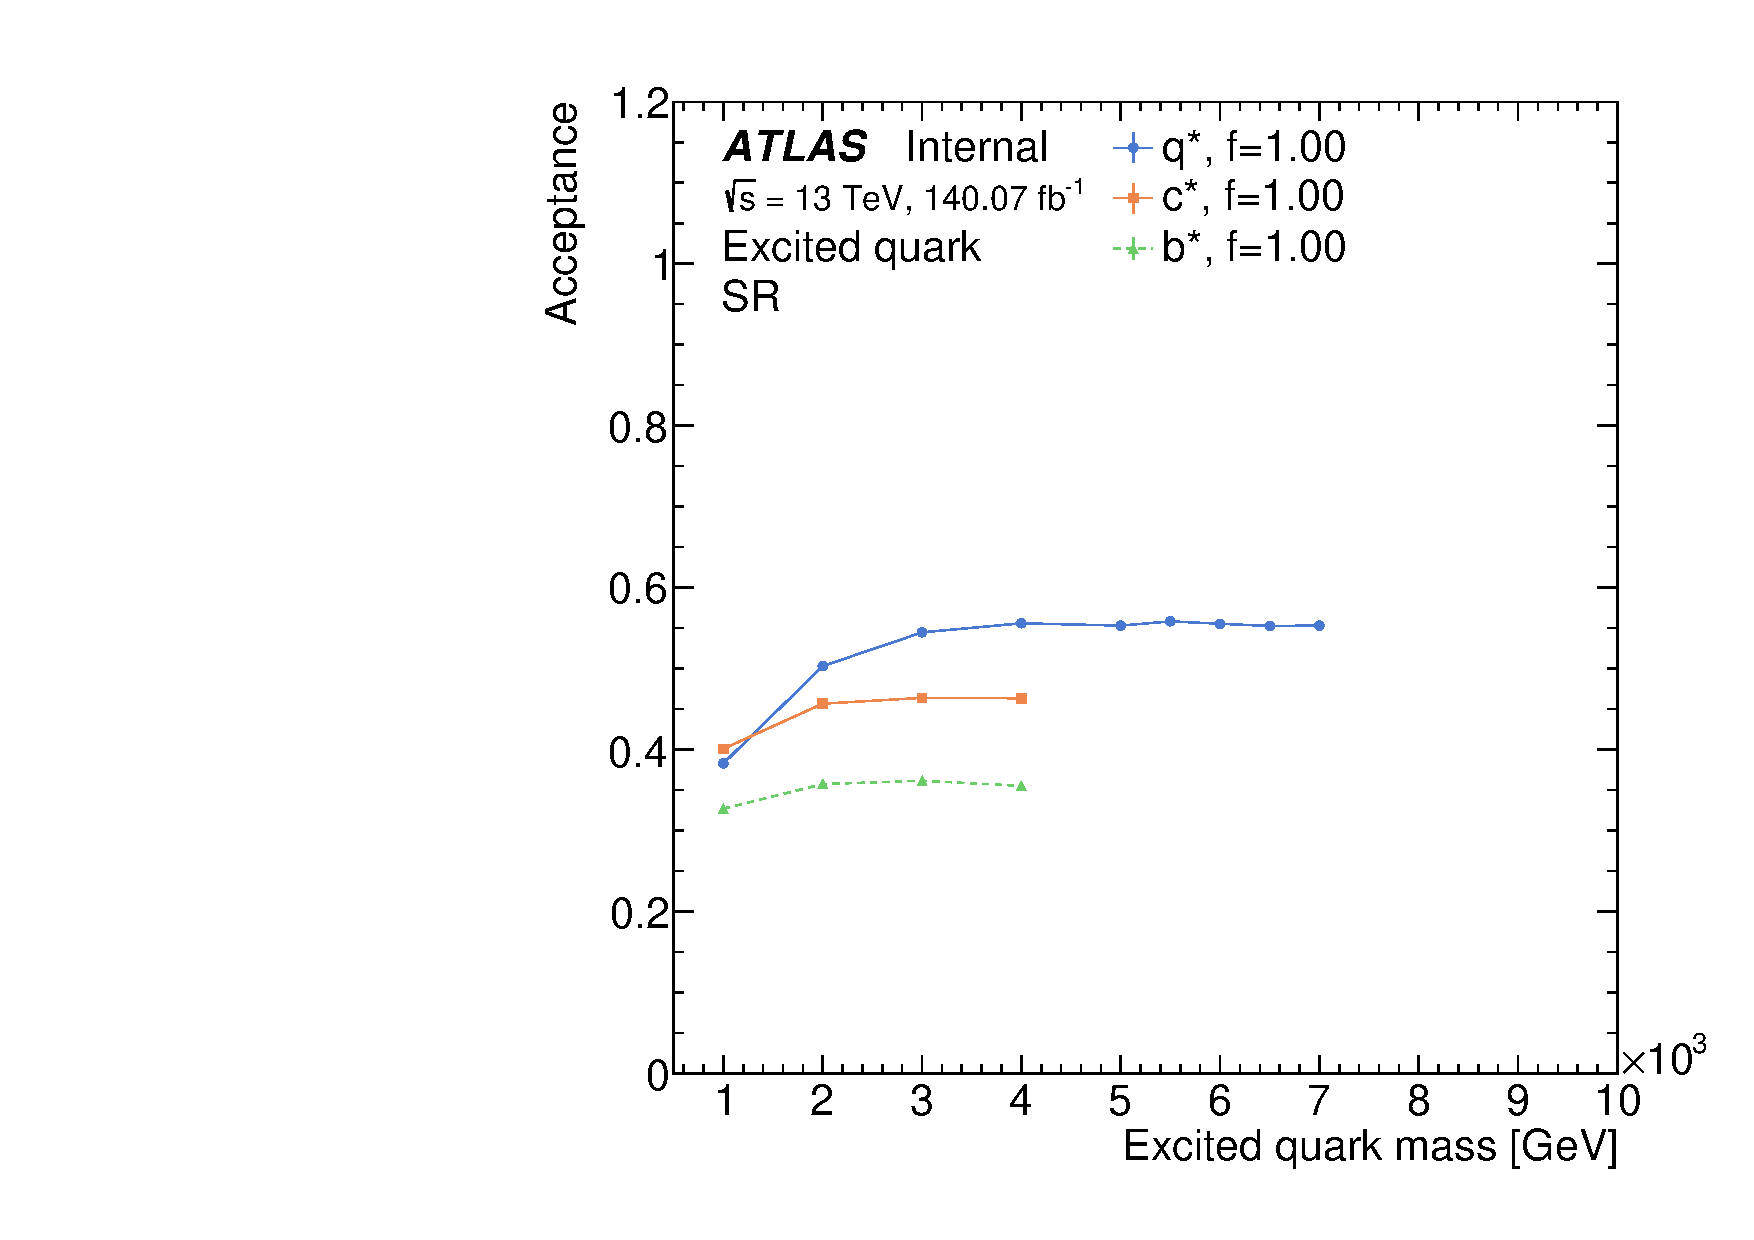
\includegraphics[width=\linewidth]{5_resonances/signal/acceptances/qstar/can__bStar__coupling_comparison__phjet_m_acceptance}
        \caption{\ac{EQ}}
        \label{fig:signals:acc_eff:acceptances:qstar}
    \end{subfigure}
    \hfill
    \begin{subfigure}[h]{0.49\linewidth}
        \centering
        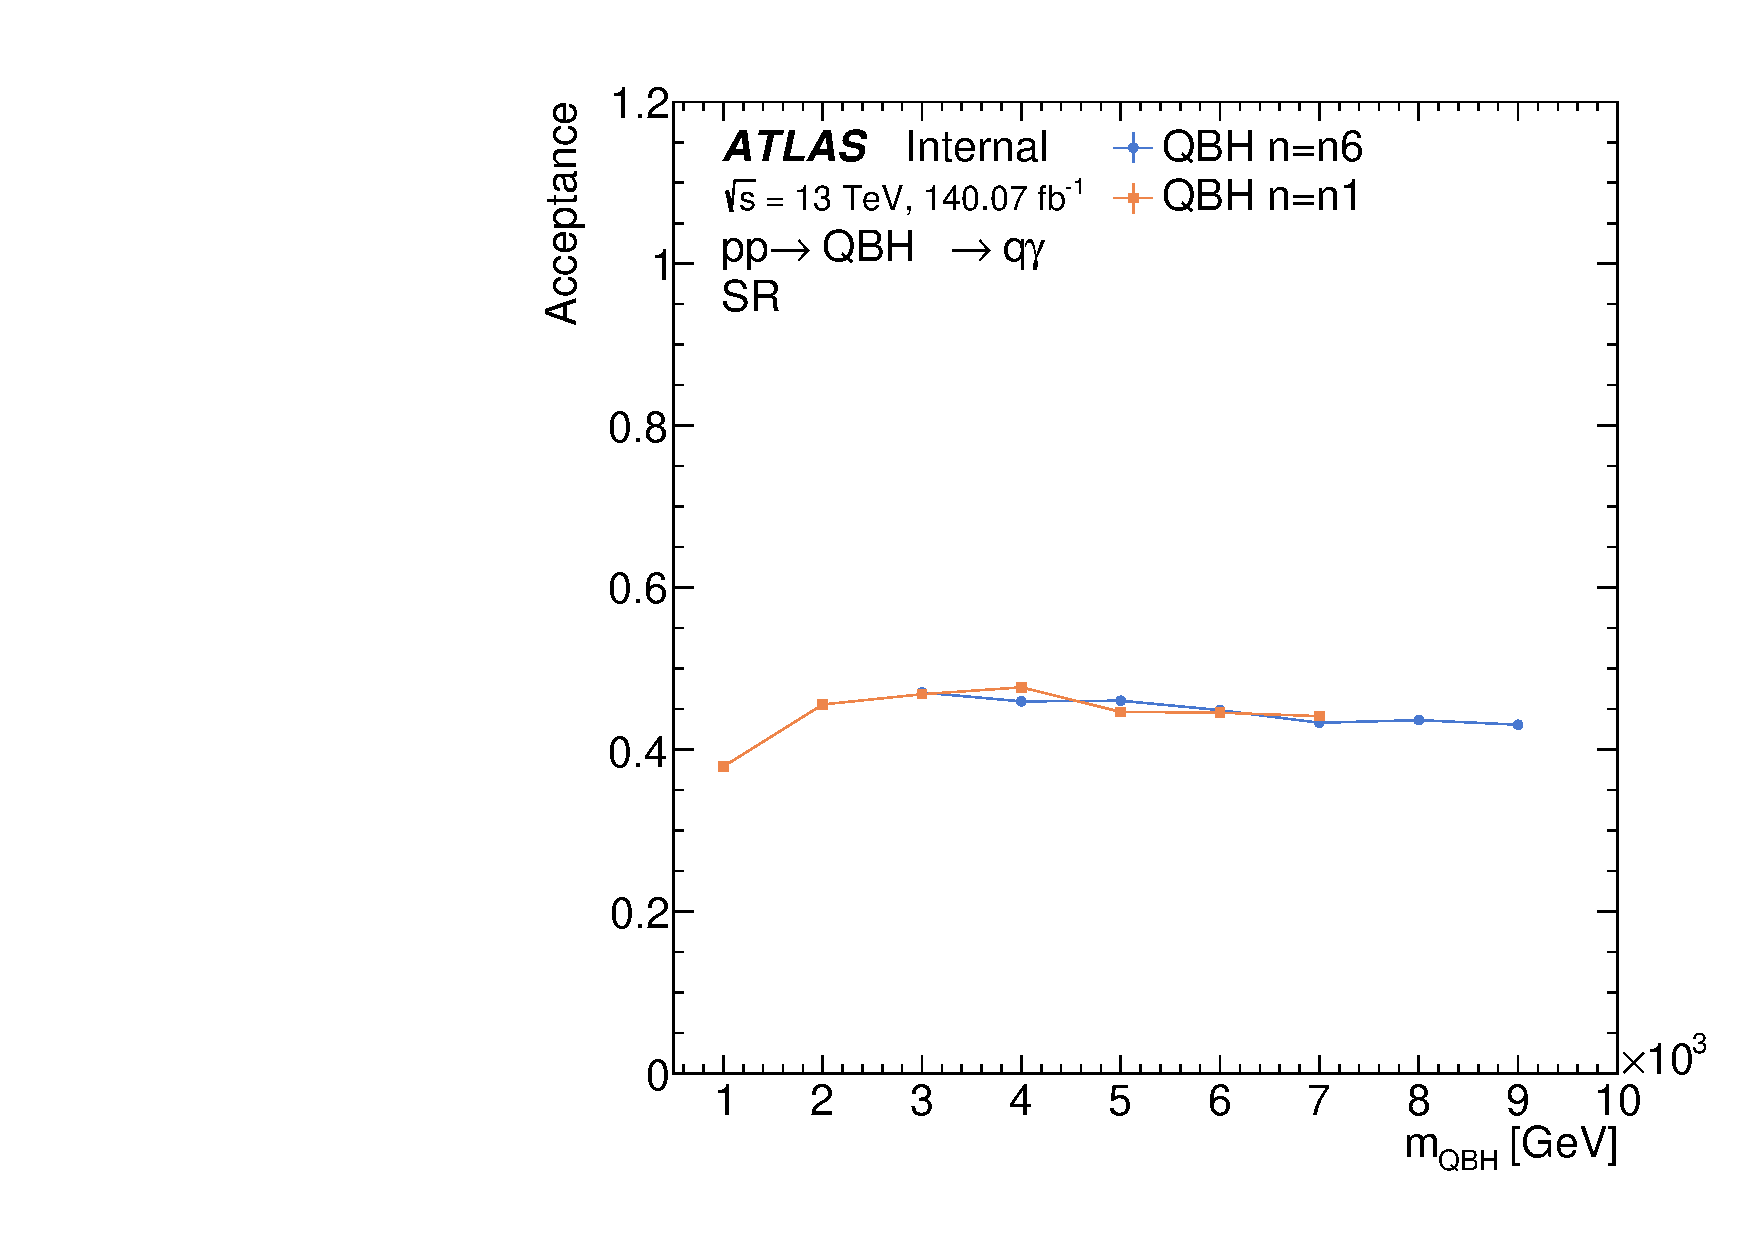
\includegraphics[width=\linewidth]{5_resonances/signal/acceptances/QBH/can__QBH_n1__phjet_m_acceptance}
        \caption{\ac{QBH}}
        \label{fig:signals:acc_eff:acceptances:qbh}
    \end{subfigure}
    \caption{Measured acceptances for the \ac{EQ} (left) and \ac{QBH} (right).}
    \label{fig:signals:acc_eff:acceptances}
\end{figure}

\begin{figure}[ht!]
    \centering
    \begin{subfigure}[h]{0.32\linewidth}
        \centering
        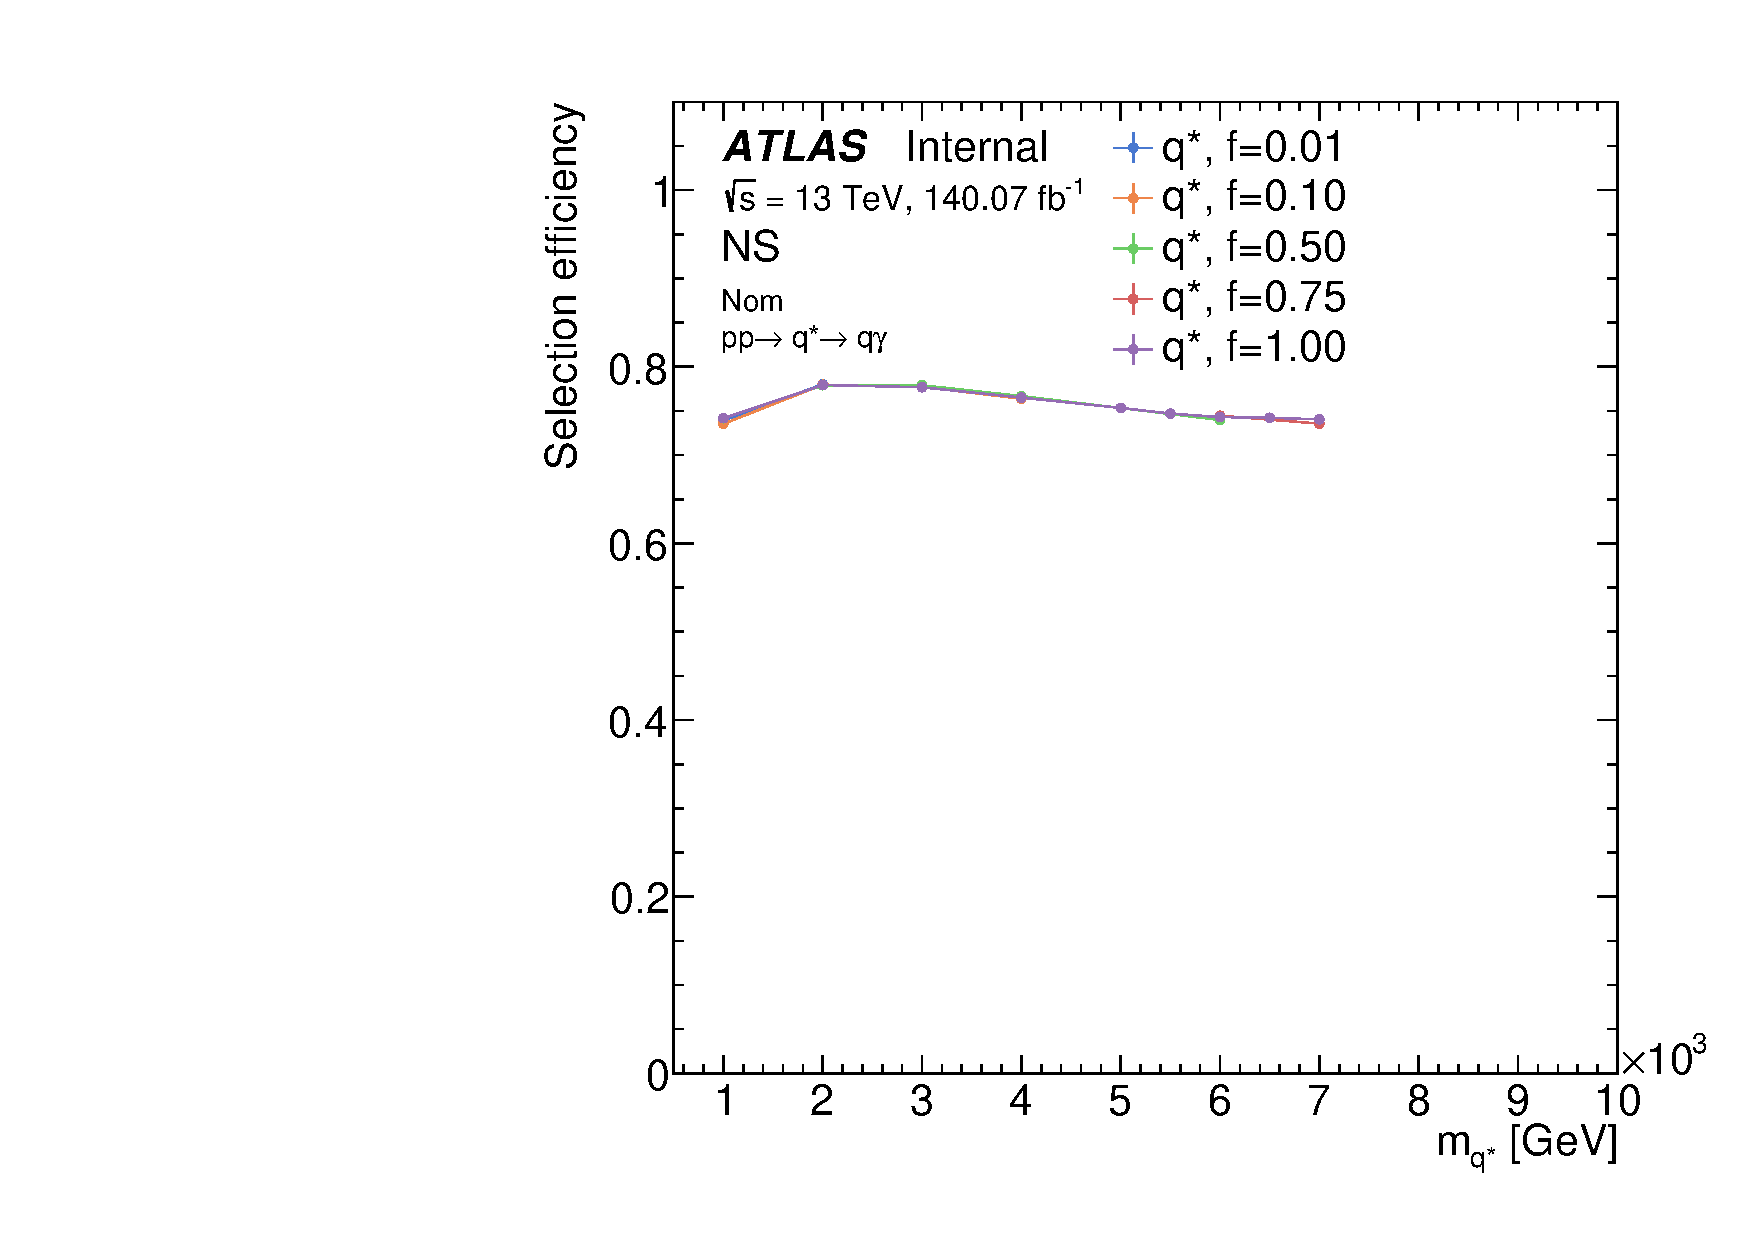
\includegraphics[width=\linewidth]{5_resonances/signal/efficiencies/NS/sig/full_efficiencies/NOM/Nom/qstar/can__qStar__Nom__NS__efficiency}
        \caption{\qstar signals in no-tag region.}
        \label{fig:signals:acc_eff:efficiencies:qstar}
    \end{subfigure}
    \hfill
    \begin{subfigure}[h]{0.32\linewidth}
        \centering
        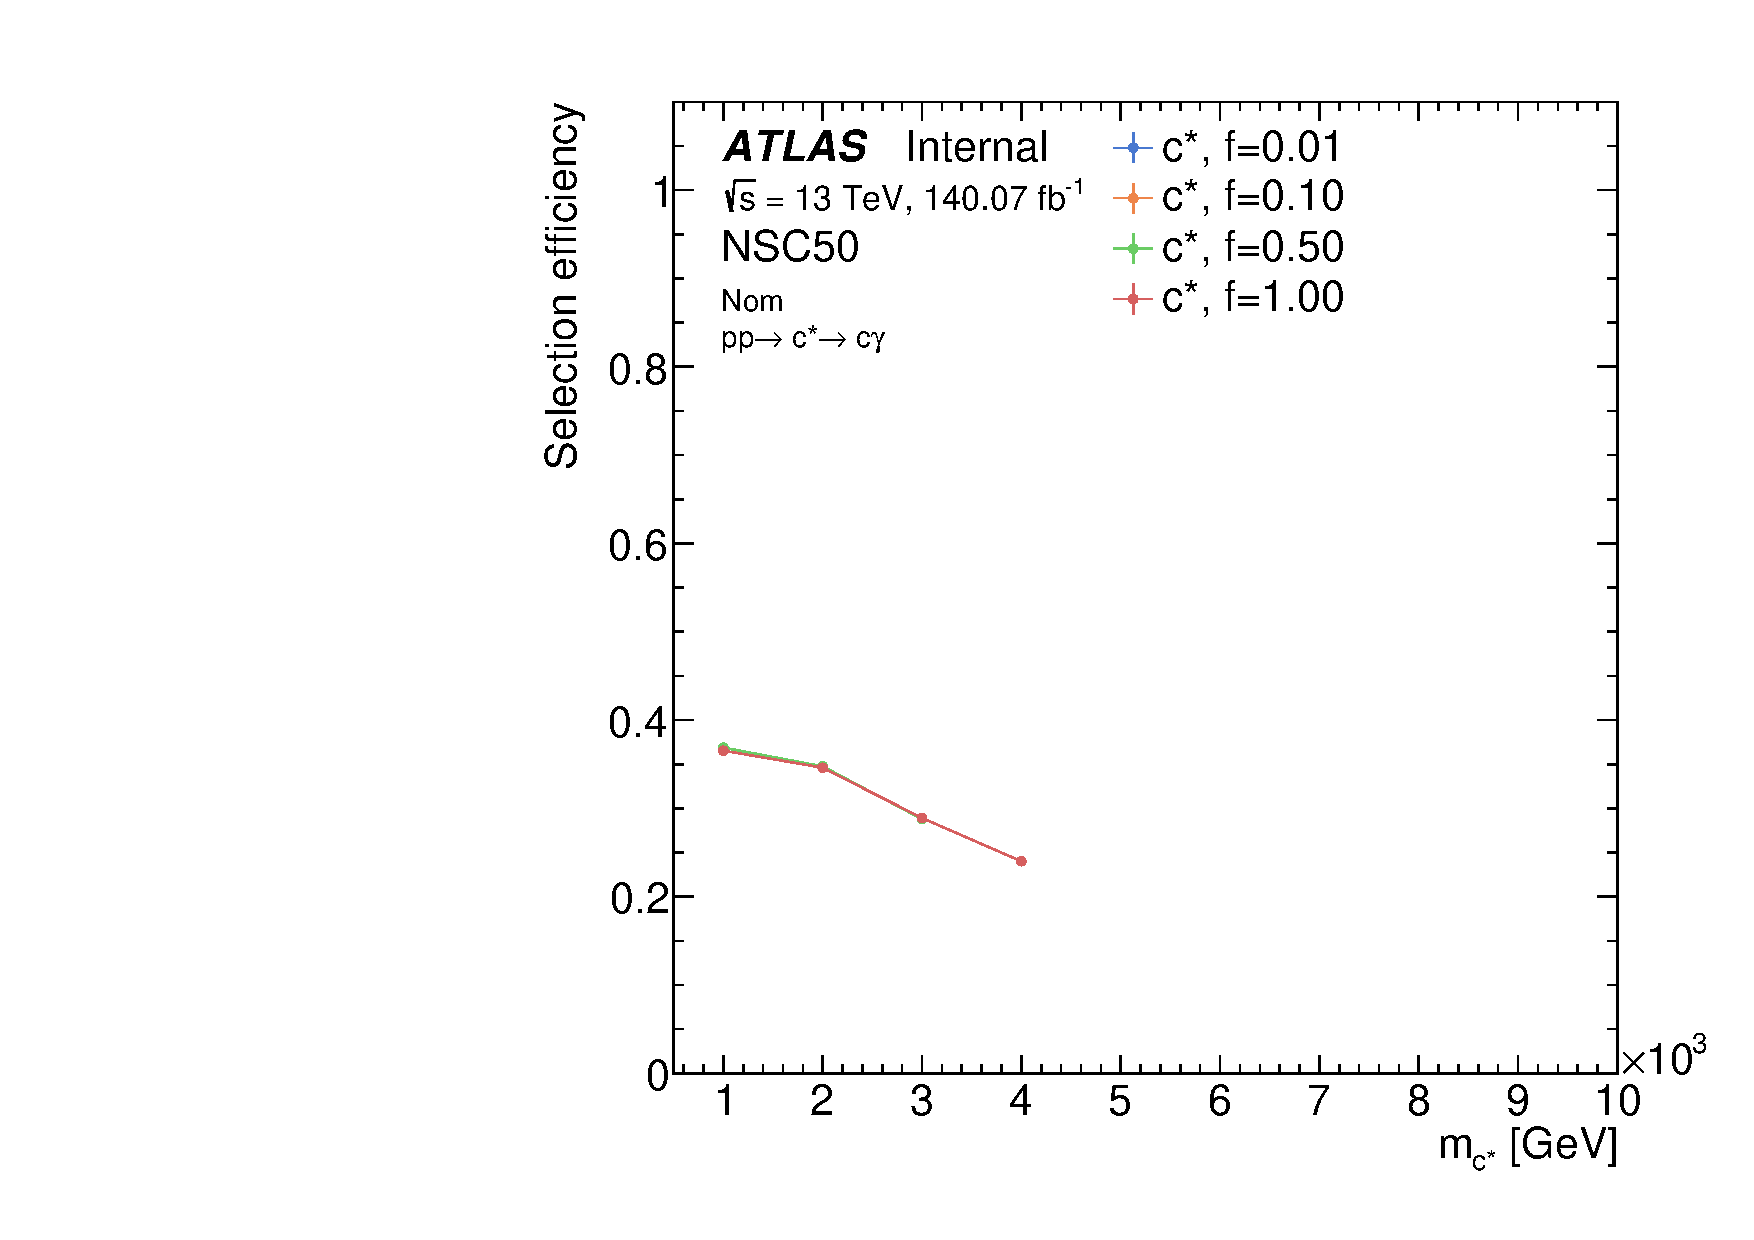
\includegraphics[width=\linewidth]{5_resonances/signal/efficiencies/NSC50/sig/full_efficiencies/NOM/Nom/qstar/can__cStar__Nom__NSC50__efficiency}
        \caption{\cstar in \ctagged region.}
        \label{fig:signals:acc_eff:efficiencies:cstar}
    \end{subfigure}
    \hfill
    \begin{subfigure}[h]{0.32\linewidth}
        \centering
        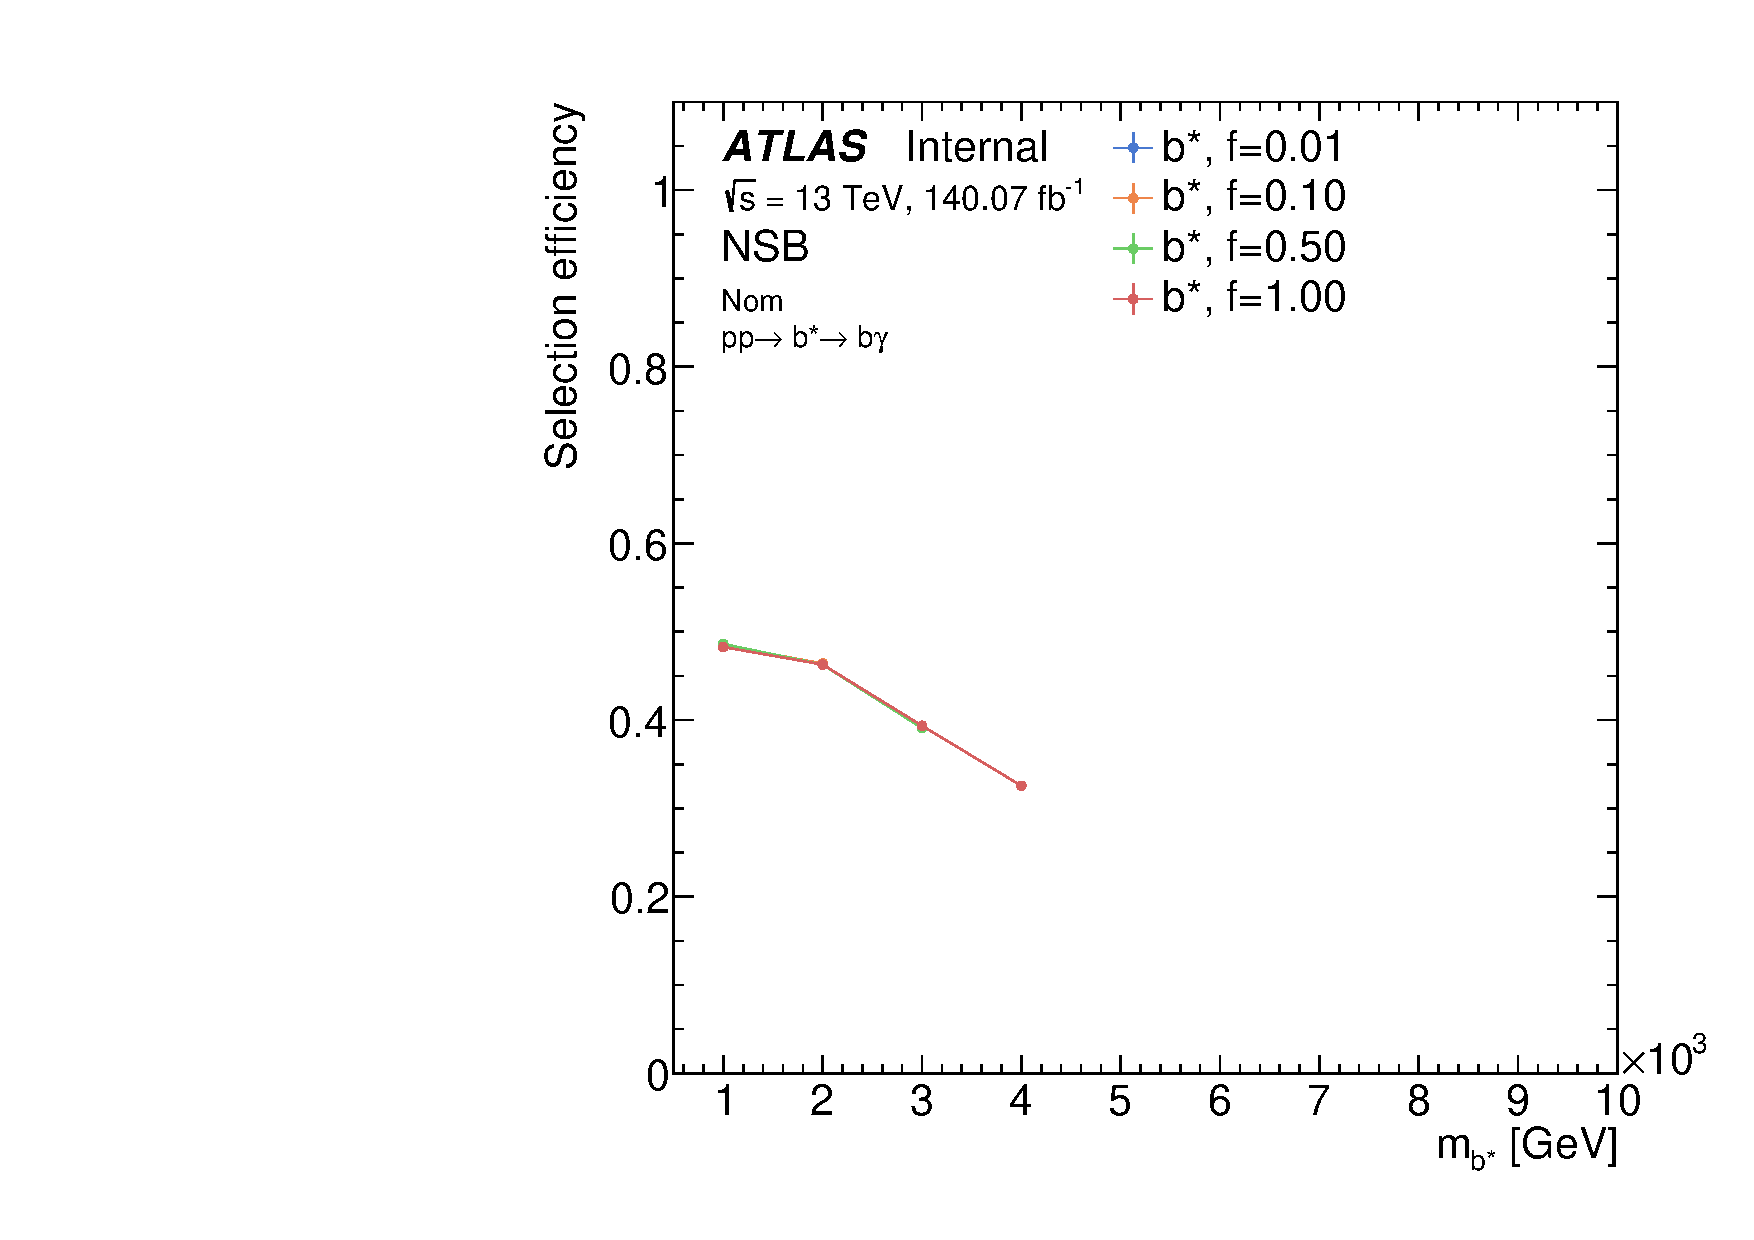
\includegraphics[width=\linewidth]{5_resonances/signal/efficiencies/NSB/sig/full_efficiencies/NOM/Nom/qstar/can__bStar__Nom__NSB__efficiency}
        \caption{\bstar in \btagged region.}
        \label{fig:signals:acc_eff:efficiencies:bstar}
    \end{subfigure}
    \caption{Measured efficiencies for the \ac{EQ} signals. \Fig{\subref{fig:signals:acc_eff:efficiencies:qstar}}: \qstar signal when no tagging is applied whatsoever; \Fig{\subref{fig:signals:acc_eff:efficiencies:cstar}}: \cstar signal with \ctagging applied; and \Fig{\subref{fig:signals:acc_eff:efficiencies:bstar}}: \bstar signal with \btagging applied.}
    \label{fig:signals:acc_eff:efficiencies}
\end{figure}







%%%%%%%%%%%%%%%%%%%%%%%%%%%%%%%%%%%%%%%%%%%%%%%%%%%%%%%%%%%%%%%%%%%%%%%%%%%%%%%%%%%%%%%%%%%%%%%%%%%%
%%%%%%%%%%%%%%%%%%%%%%%%%%%%%%%%%%%%%%%%%%%%%%%%%%%%%%%%%%%%%%%%%%%%%%%%%%%%%%%%%%%%%%%%%%%%%%%%%%%%
%%%%%%%%%%%%%%%%%%%%%%%%%%%%%%%%%%%%%%%%%%%%%%%%%%%%%%%%%%%%%%%%%%%%%%%%%%%%%%%%%%%%%%%%%%%%%%%%%%%%
%%%%%%%%%%%%%%%%%%%%%%%%%%%%%%%%%%%%%%%%%%%%%%%%%%%%%%%%%%%%%%%%%%%%%%%%%%%%%%%%%%%%%%%%%%%%%%%%%%%%
%%%%%%%%%%%%%%%%%%%%%%%%%%%%%%%%%%%%%%%%%%%%%%%%%%%%%%%%%%%%%%%%%%%%%%%%%%%%%%%%%%%%%%%%%%%%%%%%%%%%
%%%%%%%%%%%%%%%%%%%%%%%%%%%%%%%%%%%%%%%%%%%%%%%%%%%%%%%%%%%%%%%%%%%%%%%%%%%%%%%%%%%%%%%%%%%%%%%%%%%%









%%%%%%%%%%%%%%%%%%%%%%%%%%%%%%%%%%%%%%%%%%%%%%%%%%%%%%%%%%%%%%%%%%%%%%%%%%%%%%%%%%%%%%%%%%%%%%%%%%%%
%%%%%%%%%%%%%%%%%%%%%%%%%%%%%%%%%%%%%%%%%%%%%%%%%%%%%%%%%%%%%%%%%%%%%%%%%%%%%%%%%%%%%%%%%%%%%%%%%%%%
%%%%%%%%%%%%%%%%%%%%%%%%%%%%%%%%%%%%%%%%%%%%%%%%%%%%%%%%%%%%%%%%%%%%%%%%%%%%%%%%%%%%%%%%%%%%%%%%%%%%
%%%%%%%%%%%%%%%%%%%%%%%%%%%%%%%%%%%%%%%%%%%%%%%%%%%%%%%%%%%%%%%%%%%%%%%%%%%%%%%%%%%%%%%%%%%%%%%%%%%%
%%%%%%%%%%%%%%%%%%%%%%%%%%%%%%%%%%%%%%%%%%%%%%%%%%%%%%%%%%%%%%%%%%%%%%%%%%%%%%%%%%%%%%%%%%%%%%%%%%%%
%%%%%%%%%%%%%%%%%%%%%%%%%%%%%%%%%%%%%%%%%%%%%%%%%%%%%%%%%%%%%%%%%%%%%%%%%%%%%%%%%%%%%%%%%%%%%%%%%%%%
\section{Systematic uncertainties}
\label{sec:signals:systs}

Systematic uncertainties are one of the most crucial aspects in a search, given that they modify the signal expected values in the different signal regions of the analysis. These uncertainties are included in the statistical model as nuisance parameters, explained in \Sect{\ref{subsec:strategy:stat_treatment:systs}}.
As in this analysis the background is obtained directly from data, systematic uncertainties only enter the statistical model through the signals. However, uncertainties related to the background modeling are still taken into account, but a speciific estimation of those is given in \Ch{\ref{ch:bkg}}. 
There are two types of systematic uncertainties affecting the signals: experimental and theoretical, and both are described in the following.


% In the present work, systematic uncertainties arise from the reconstruction of the various physics objects, from theoretical and modelling uncertainties affecting the predictions of the signals. These uncertainties manifest themselves as uncertainties in the overall yield of the final observable. The uncertainties are grouped in two categories, depending what they affect:
% \begin{itemize}
%     \item Signal uncertainties: they comprise uncertainties that will affect the signal shape or yield. There are three sources:
%         \begin{itemize}
%             \item Detector or experimental uncertainties.
%             \item Theory/modelling uncertainties.
%         \end{itemize}
%     \item Background modeling uncertainties: they are uncertainties associated with the choice of the fit function.
% \end{itemize}

% In the following sections, a detailed description of each source of uncertainty will be shown.


%%%%%%%%%%%%%%%%%%%%%%%%%%%%%%%%%%%%%%%%%%%%%%%%%%%%%%%%%%%%%%%%%%%%%%%%%%%%%%%%%%%%%%%%%%%%%%%%%%%%
%%%%%%%%%%%%%%%%%%%%%%%%%%%%%%%%%%%%%%%%%%%%%%%%%%%%%%%%%%%%%%%%%%%%%%%%%%%%%%%%%%%%%%%%%%%%%%%%%%%%
%%%%%%%%%%%%%%%%%%%%%%%%%%%%%%%%%%%%%%%%%%%%%%%%%%%%%%%%%%%%%%%%%%%%%%%%%%%%%%%%%%%%%%%%%%%%%%%%%%%%
\subsection{Experimental uncertainties}
\label{subsec:signals:systs:exp}

Experimental uncertainties arise from uncertainties on the simulation of the detector, reconstruction or calibration of physical objects, corrections due to pileup or luminosity.

For each one of the considered sources of uncertainties, with the exception of the luminosity ones, their effect is studied on the relative difference seen on the selection efficiency of the signals.

% In the following, a description of the procedures to evaluate uncertainties common to all processes are discussed. The prescription and tools are those implemented in the \texttt{SUSYTools} package used in this analysis. For each one of the uncertainties considered, the effects of the uncertainty are studied in terms of the relative uncertainty on the selection efficiency of the signals. %Furthermore, the relative uncertainties on the mean and standard deviation of the signals for each variation are computed and are shown in \App{\ref{app:systs_means_stddevs}}

\subsubsection{Luminosity and pileup reweighting uncertainty}
The uncertainty on the combined full Run-2 integrated luminosity is obtained using the LUCID-2 detector \cite{ATLAS-LUCID2} for the primary luminosity measurements, complemented by measurements using the \ac{ID} and calorimeters. The obtained uncertainty is of \(0.83\%\) \cite{ATLAS-Lumi-Run2}. 
Moreover, uncertainties related to the reweighting of \ac{MC} events to match the pile-up distributions found in data need to be taken into account for which a nuisance parameter is added to the fit, allowing for variations of the applied pile-up event weight~\cite{ATLAS-PileupRW}.


\subsubsection{Photon identification, isolation, trigger, energy scale and resolution}
The uncertainty on the photon identification is evaluated by computing the difference between identification efficiencies by applying the uncertainties on the photon \ac{FF}, computed in \Ch{\ref{ch:ss_corrections}}.
Regarding the uncertainties on photon isolation, they are computed by applying data-driven shifts to the simulated \etiso shapes. The effect of these uncertainties on the selection efficiency is fount to be, in all cases, \(<0.2\%\).
The photon energy scale and resolution is considered as well, and the uncertainties are found to be \(<0.5\%\).

% {
%     \color{red}
%     For the current version of results, the identification, isolation and trigger scale factors are set to \(1\), and a fixed, conservative, uncertainty of \(5\%\) is used. This is because the presented efficiencies variations correspond to using the \texttt{AnalysisBase} release 21.2. Once final release 22 recommendations are released, the correct configuration will be used.
% }


\subsubsection{Jet energy scale (JER) and resolution (JES)}

The uncertainties associated with jets are estimated following the methodology described in \Refns{\cite{ATLAS-JetEnergy-2011}}{\cite{ATLAS-JESJERMC-2015}}, which come from multiple sources and provide a large number of nuisance parameters.
Among them are the uncertainty associated with the energy resolution (JER), obtained from the variation in the smearing of the \ac{MC} jets to the data to correct the \ac{MC} resolution. These uncertainties are evaluated from dijet events and zero bias data using random cones. 
The uncertainties related to the energy scale (JES) arise from dijet eta-intercalibration across eta, \(\Zboson\left(\ra ee, \mu\mu\right)\)+jets, \gammajet and multijet balance, and the propagation of single particles in high-\pt regimes.
The uncertainties due to the mistag rate of the pileup suppression algorithm (mistakenly tagging hard scattering jets) and the impact of the MC generator are also taken into account.
It is found that the jet uncertainties are no bigger than \(0.1\%\).

% {
%     \color{red}
%     With the newest jet uncertainties configuration file \\
%     \texttt{rel22/Summer2024\_PreRec/R4\_CategoryReduction\_Phase1\_FullJER.config}, an extra uncertainty dedicated to \textsc{AtlasFast3} signals will be added.
% }



\subsubsection{Jet flavour tagging}

This analysis heavily relies on the identification of \bjets and \cjets. All of the employed heavy-flavor tagging algorithms entail systematic uncertainties which need to be considered. The \btagging uncertainties are given as a reduced nuisance parameter set consisting of scale factor uncertainties for \btagging efficiency, \cjet mistag rate, \ljet mistag rate and high-\pt extrapolation. Given that the final calculations are not ready yet, a fixed and very conservative \(30\%\) uncertainty is considered in every flavour-tagged region of the analysis.


% To take into account flavour mis-tagging, a fixed \(30\%\) uncertainty on the selection efficiency is set for each flavour. The reason to have a very conservative and fixed uncertainty is the fact that final calculations 

% Flavour tagging uncertainties are considered  (\texttt{FT\_EFF\_\{B,C,Light\},FT\_EFF\_extrapolation\{charm\}}) are \(\pm 1 \sigma\) variations in the error on the scale factor that corrects the tagging rate in simulation to match the one in data.
% {
%     \color{red}
%     Final recommendations for the GN2v01 tagger are not ready yet, therefore a fixed uncertainty for all flavors is set to \(30\%\).
% }

% The effect on the relative uncertainty on the selection efficiency is displayed in \Fig{\ref{fig:systematics:jetw_relunc_qstar}}.









% A summary of the experimental systematic uncertainties taken into account in this analysis is given in \Tab{\ref{tab:systematics:syst_summary_sources}}, along with the shorthand name of the uncertainty used throughout the analysis and whether they affect kinematics or weights of the event or object.
% %% \textit{Include also subsections for each of the individual descriptions of the uncertainty groups and the source where they come from.  If the recommendation is not available at this time, state that in the section.}

% \begin{table}[ht]
%     \centering
%     \scriptsize
%     \begin{center}
%         \begin{tabular}{lll}
%             \toprule \midrule
%             Systematic uncertainty & Affects weights or kinematics & Fixed value\\
%             \midrule
%             \multicolumn{3}{c}{\textbf{Event}}  \\
%             \midrule
%             Luminosity  & -   & \(0.83\%\) \\
%             \midrule
%             \multicolumn{3}{c}{\textbf{Photons} - \fixme{list not final, waiting for EGamma Rel22 recommendations}}  \\
%             \midrule
%             \texttt{PH\_EFF\_Trigger\_TOTAL\_1NPCOR\_PLUS\_UNCOR}   & weights    & \(5\%\)\\
%             \texttt{PH\_EFF\_ID\_Uncertainty}                       & weights    & \(5\%\)\\
%             \texttt{PH\_EFF\_Iso\_Uncertainty}                      & weights    & \(5\%\)\\
%             \texttt{EG\_SCALE\_ALL}                                 & kinematics & \\
%             \texttt{EG\_SCALE\_AF2}                                 & kinematics & \\
%             \texttt{EG\_RESOLUTION\_ALL}                            & kinematics & \\
%             \midrule
%             \multicolumn{3}{c}{\textbf{Jets} - \fixme{list not final, waiting for Jet/Etmiss Rel22 recommendations}}  \\
%             \midrule
%             \texttt{JET\_JERUnc\_Noise\_PreRec}                                           & kinematics &  \\
%             \texttt{JET\_JERUnc\_mc20vsmc21\_MC20\_PreRec}                                & kinematics &  \\
%             \texttt{JET\_JER\_DataVsMC\_MC16}                                             & kinematics &  \\
%             \texttt{JET\_JER\_EffectiveNP\_\{1,2,3,4,5,6,7,8,9,10,11,12restTerm\}}        & kinematics &  \\
%             \texttt{JET\_BJES\_Response}                                                  & kinematics &  \\
%             \texttt{JET\_EffectiveNP\_Detector\{1,2\}}                                    & kinematics &  \\
%             \texttt{JET\_EffectiveNP\_Mixed\{1,2\}}                                       & kinematics &  \\
%             \texttt{JET\_EffectiveNP\_Modelling\{1,2,3\}}                                 & kinematics &  \\
%             \texttt{JET\_EffectiveNP\_Statistical\{1,2,3,4\}}                             & kinematics &  \\
%             \texttt{JET\_EtaIntercalibration\_\{Modelling,NonClosure\_PreRec,TotalStat\}} & kinematics &  \\
%             \texttt{JET\_Flavor\_Composition}                                             & kinematics &  \\
%             \texttt{JET\_Flavor\_Response}                                                & kinematics &  \\
%             \texttt{JET\_InSitu\_NonClosure\_PreRec}                                      & kinematics &  \\
%             \texttt{JET\_JESUnc\_Noise\_PreRec}                                           & kinematics &  \\
%             \texttt{JET\_JESUnc\_VertexingAlg\_PreRec}                                    & kinematics &  \\
%             \texttt{JET\_JESUnc\_mc20vsmc21\_MC20\_PreRec}                                & kinematics &  \\
%             \texttt{JET\_Pileup\_OffsetMu}                                                & kinematics &  \\
%             \texttt{JET\_Pileup\_OffsetNPV}                                               & kinematics &  \\
%             \texttt{JET\_Pileup\_PtTerm}                                                  & kinematics &  \\
%             \texttt{JET\_Pileup\_RhoTopology}                                             & kinematics &  \\
%             \texttt{JET\_PunchThrough\_MC16}                                              & kinematics &  \\
%             \texttt{JET\_SingleParticle\_HighPt}                                          & kinematics &  \\
%             \texttt{JET\_JvtEfficiency}                                                   & weights    &  \\
%             \midrule
%             \multicolumn{3}{c}{\textbf{Flavour tagging} - \fixme{list not final, waiting for FTAG recommendations}}  \\
%             \midrule
%             \texttt{FT\_EFF}                          & weights  & \(30\%\) \\
%             % \texttt{FT\_EFF\_B}                          & weights \\
%             % \texttt{FT\_EFF\_C}                          & weights \\
%             % \texttt{FT\_EFF\_Light}                      & weights \\
%             % \texttt{FT\_EFF\_EIGEN\_extrapolation}              & weights \\
%             % \texttt{FT\_EFF\_EIGEN\_extrapolation\_from\_charm} & weights \\
%             \midrule
%             \midrule
%             \texttt{PRW\_DATASF}         & weights & \\
%             \bottomrule
%         \end{tabular}
%     \end{center}
%     \caption{Qualitative summary of the experimental systematic uncertainties considered in this analysis.}
%     \label{tab:systematics:syst_summary_sources}
% \end{table}
%%%%%%%%%%%%%%%%%%%%%%%%%%%%%%%%%%%%%%%%%%%%%%%%%%%%%%%%%%%%%%%%%%%%%%%%%%%%%%%%%%%%%%%%%%%%%%%%%%%%
%%%%%%%%%%%%%%%%%%%%%%%%%%%%%%%%%%%%%%%%%%%%%%%%%%%%%%%%%%%%%%%%%%%%%%%%%%%%%%%%%%%%%%%%%%%%%%%%%%%%
%%%%%%%%%%%%%%%%%%%%%%%%%%%%%%%%%%%%%%%%%%%%%%%%%%%%%%%%%%%%%%%%%%%%%%%%%%%%%%%%%%%%%%%%%%%%%%%%%%%%



%%%%%%%%%%%%%%%%%%%%%%%%%%%%%%%%%%%%%%%%%%%%%%%%%%%%%%%%%%%%%%%%%%%%%%%%%%%%%%%%%%%%%%%%%%%%%%%%%%%%
%%%%%%%%%%%%%%%%%%%%%%%%%%%%%%%%%%%%%%%%%%%%%%%%%%%%%%%%%%%%%%%%%%%%%%%%%%%%%%%%%%%%%%%%%%%%%%%%%%%%
%%%%%%%%%%%%%%%%%%%%%%%%%%%%%%%%%%%%%%%%%%%%%%%%%%%%%%%%%%%%%%%%%%%%%%%%%%%%%%%%%%%%%%%%%%%%%%%%%%%%
\subsection{Theory uncertainties}
\label{subsec:signals:systs:theo}

The \ac{EQ} models determined from \ac{MC} simulations are subject to theoretical uncertainties. Three sources of uncertainty are evaluated, and described in the following.

The effect of missing higher orders in the calculation of the hard interaction is estimated by varying the factorization and renormalization scales for \ac{QCD} emissions in \ac{FSR} and \ac{ISR} by \(\{0.5, 0.625, 0.75, 0.875, 1.0, 1.25, 1.75, 2.0\}\) \fixme{change to 7?}, leading to a total of 20 combinations. The scale uncertainty is then approximated by adding in quadrature each one of these variations \fixme{need to change to envelope?}. This corresponds to the biggest theoretical uncertainty, having a magnitude of at most \(2\%\).

The \ac{PDF1} uncertainty is estimated using 100 alternative replicas of the \ac{PDF1}. These are provided by the NNPDF group~\cite{NNPDF2} and encode uncertainties on the measurements entering the \ac{PDF1} fit and the fitting method. The \ac{PDF1} uncertainty is given by the standard deviation over the replica sample. In this analysis, it is found to be \(<1\%\).

Finally, \fixme{finish with alphaS uncertainties, asked about how it's done}

Regarding theoretical uncertainties for the \ac{QBH} samples is less motivated than that for \acp{EQ}, given that none of the \acp{PDF1} includes the effects of gravity and the \ac{QCD} scale for strong gravity is unknown.
%%%%%%%%%%%%%%%%%%%%%%%%%%%%%%%%%%%%%%%%%%%%%%%%%%%%%%%%%%%%%%%%%%%%%%%%%%%%%%%%%%%%%%%%%%%%%%%%%%%%
%%%%%%%%%%%%%%%%%%%%%%%%%%%%%%%%%%%%%%%%%%%%%%%%%%%%%%%%%%%%%%%%%%%%%%%%%%%%%%%%%%%%%%%%%%%%%%%%%%%%
%%%%%%%%%%%%%%%%%%%%%%%%%%%%%%%%%%%%%%%%%%%%%%%%%%%%%%%%%%%%%%%%%%%%%%%%%%%%%%%%%%%%%%%%%%%%%%%%%%%%


%%%%%%%%%%%%%%%%%%%%%%%%%%%%%%%%%%%%%%%%%%%%%%%%%%%%%%%%%%%%%%%%%%%%%%%%%%%%%%%%%%%%%%%%%%%%%%%%%%%%
%%%%%%%%%%%%%%%%%%%%%%%%%%%%%%%%%%%%%%%%%%%%%%%%%%%%%%%%%%%%%%%%%%%%%%%%%%%%%%%%%%%%%%%%%%%%%%%%%%%%
%%%%%%%%%%%%%%%%%%%%%%%%%%%%%%%%%%%%%%%%%%%%%%%%%%%%%%%%%%%%%%%%%%%%%%%%%%%%%%%%%%%%%%%%%%%%%%%%%%%%
%%%%%%%%%%%%%%%%%%%%%%%%%%%%%%%%%%%%%%%%%%%%%%%%%%%%%%%%%%%%%%%%%%%%%%%%%%%%%%%%%%%%%%%%%%%%%%%%%%%%
%%%%%%%%%%%%%%%%%%%%%%%%%%%%%%%%%%%%%%%%%%%%%%%%%%%%%%%%%%%%%%%%%%%%%%%%%%%%%%%%%%%%%%%%%%%%%%%%%%%%
%%%%%%%%%%%%%%%%%%%%%%%%%%%%%%%%%%%%%%%%%%%%%%%%%%%%%%%%%%%%%%%%%%%%%%%%%%%%%%%%%%%%%%%%%%%%%%%%%%%%